\chapter{Architecture globale}

Le projet consiste à construire une bibliothèque permettant de générer plusieurs
types de cartes d'élévations (planes, sphériques) à l'aide de diverses
méthodes (fractales, bruits), de générer leurs texture associées, de les
importer et exporter dans différents formats et enfin de les visualiser.

La figure \ref{fig:class-diagram} présente l'architecture que nous avons imaginé,
elle sera décrite plus en détails dans le chapitre suivant.

\begin{sidewaysfigure}
  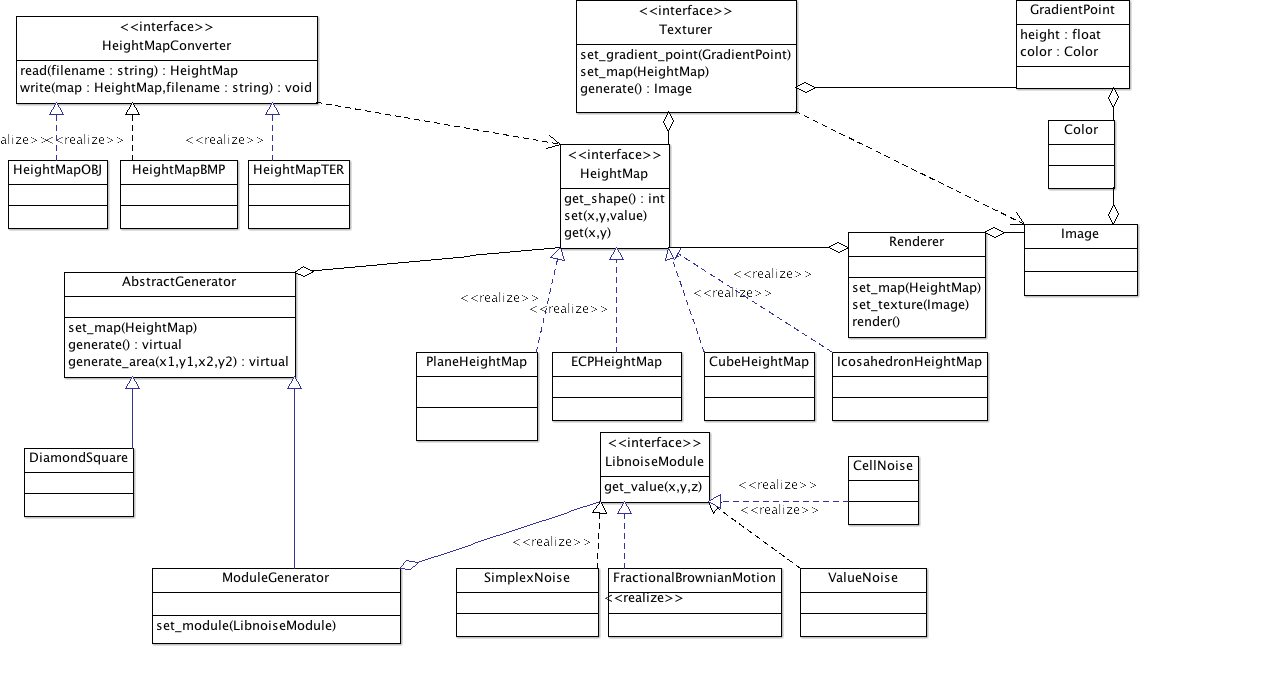
\includegraphics[width=28cm]{resources/class-diagram.png}
        \caption{Diagramme de classe}
        \label{fig:class-diagram}
\end{sidewaysfigure}
